\documentclass[12pt,fleqn,answers]{exam}
\usepackage{pifont}
\usepackage{dingbat}
\usepackage{amsmath,amssymb}
\usepackage{epsfig}
\usepackage[]{hyperref}
\usepackage{geometry}
\geometry{letterpaper, margin=0.5in}
\addpoints
\boxedpoints
\pointsinmargin
\pointname{pts}

\usepackage[activate={true,nocompatibility},final,tracking=true,kerning=true,factor=1100,stretch=10,shrink=10]{microtype}
\usepackage[american]{babel}
%\usepackage[T1]{fontenc}
\usepackage{fourier}
\usepackage{isomath}
\usepackage{upgreek,amsmath}
\usepackage{amssymb}

\newcommand{\dotprod}{\, {\scriptzcriptztyle
    \stackrel{\bullet}{{}}}\,}

\newcommand{\reals}{\mathbf{R}}
\newcommand{\lub}{\mathrm{lub}} 
\newcommand{\glb}{\mathrm{glb}} 
\newcommand{\complex}{\mathbf{C}}
\newcommand{\dom}{\mbox{dom}}
\newcommand{\cover}{{\mathcal C}}
\newcommand{\integers}{\mathbf{Z}}
\newcommand{\vi}{\, \mathbf{i}}
\newcommand{\vj}{\, \mathbf{j}}
\newcommand{\vk}{\, \mathbf{k}}
\newcommand{\bi}{\, \mathbf{i}}
\newcommand{\bj}{\, \mathbf{j}}
\newcommand{\bk}{\, \mathbf{k}}
\DeclareMathOperator{\Arg}{\mathrm{Arg}}
\DeclareMathOperator{\Ln}{\mathrm{Ln}}
\newcommand{\imag}{\, \mathrm{i}}
\newcommand{\range}{\mathrm{range}}
\newcommand{\ball}{\mathrm{ball}}
\newcommand{\true}{\mbox{True}}
\usepackage{graphicx}
\newcommand\AM{{\sc am}}
\newcommand\PM{{\sc pm}}
     
\newcommand{\quiz}{7}
\newcommand{\term}{Fall}
\newcommand{\due}{Saturday 8 October  at 11:59 \PM}
\begin{document}
\large
\vspace{0.1in}
\noindent\makebox[3.0truein][l]{{\bf MATH 460}}
{\bf Name:}  \\
\noindent \makebox[3.0truein][l]{\bf Homework \quiz, \term \/ \the\year}
%{\bf Row:}\hrulefill\
\vspace{0.1in}

\begin{quote}
    \fbox{I have neither given nor received unauthorized assistance on this assignment.}
    \end{quote}
\noindent  Homework    \quiz\/  has questions 1 through  \numquestions \/ with a total of  \numpoints\/  points.   
Neatly \textbf{hand write your solutions}, digitize your work, and turn it into Canvas. You do \textbf{not} need to 
use  La\TeX\,  for this assignment. This work is due \emph{\due}.

\vspace{0.1in}

%\noindent{\textbf{Link to your Overleaf work: }}\url{XXX}

\begin{questions} 



\question [5] Show that the set $[1,2)$ is not open. To do this, show that
\begin{equation*}
  \left(\exists x \in [1,2) \right) \left(\forall r \in \reals_{>0}\right) \left( \ball(x,r) \not \subset [1,2) \right).
\end{equation*}
\begin{solution}
Choose $x = 1$. Let $r \in \reals_{>0}$. To show 
that $\ball(x,r) \not \subset [1,2)$, we'll show
there is a memember of $\ball(x,r)$ that is not in $[1,2)$. 
Specifically, We
but $1-r/2 \notin [1,2)$. So $\ball(1,r) \not \subset [1,2)$.
  
\end{solution}


\question [5] Let $F$ be a convergent sequence. Show that
\begin{equation*}
  \range(F) \subset \reals_{>0} \implies \lim_{\infty} (F) \in \reals_{\geq 0}.
\end{equation*}

\begin{solution} We'll prove the contrapositive. Thus, we'll show 
  that 
  \begin{equation*}
    \lim_{\infty} F \in \reals_{< 0} \implies \range(F) \not \subset \reals_{>0}.
  \end{equation*}
  Define $\displaystyle \lim_{\infty} (F) = L$, where $L < 0$. Since $-L/2 \in \reals_{>0}$, there is
  $n \in \integers$ such that for all $k \in \integers_{>n}$, we have $F_k  \in (L + L/2, L - L/2)$;
  equivalently  $F_k  \in (3 L/2, L/2)$. In particular, $F_{n+1} < L/2 < 0$; therefore $\range(F) \not \subset 
  \reals_{>0}$

\end{solution}

  


\question [5] Give an example of a sequence $G$ such that $\range(G) \subset \reals_{>0}$ but 
$\displaystyle \lim_{\infty} G \notin \reals_{>  0}$.

\begin{solution} An example is $F = k \in \integers_{\geq 0} \mapsto 1/k$.   The proof that this
is an example is a calculus calculation.
\end{solution}

\question[5] Draw a nicely labeled picture that shows that
\begin{equation*}
  \left(\forall a \in \reals_{>-1}\right)\left(\forall x \in \reals_{>-1}\right) \left(\sqrt{1+x} \leq \sqrt{1+a} + \frac{1}{2 \sqrt{1+a}} (x-a) \right).
\end{equation*}
\textbf{Hint:}  Draw a graph of $y = \sqrt{1+x}$. On the same graph, draw a graph of the tangent line to $y = \sqrt{1+x}$
at the point $(x=a, y=\sqrt{1+a})$.

\begin{solution}

%\begin{figure}[h]
  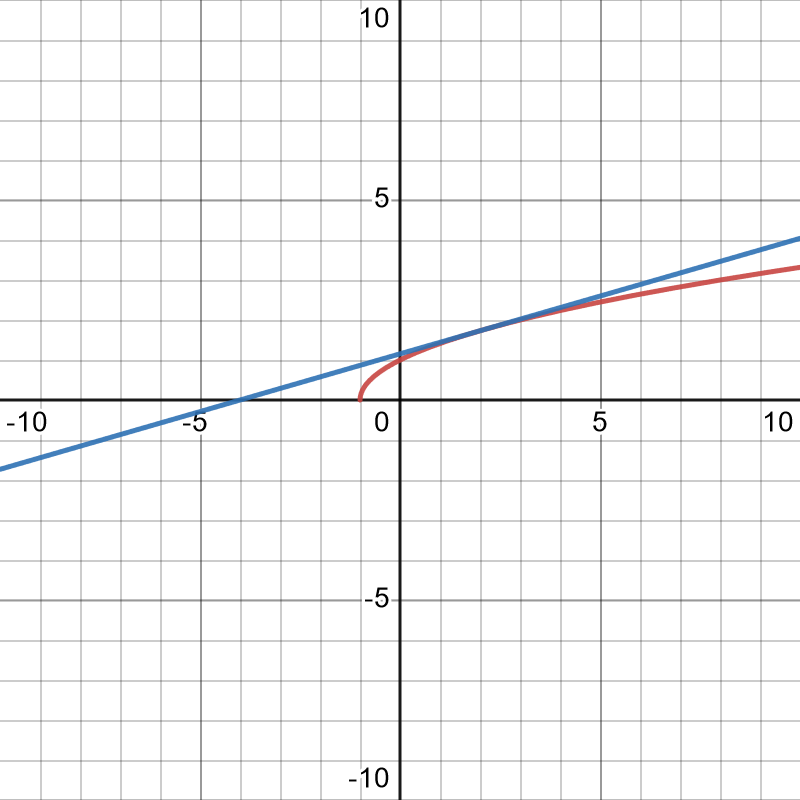
\includegraphics[scale=0.25]{desmos-graph(36).png}
 % \end{figure}
 
 This picture is specialized to $a=2$, but the picture for the general case is similar. The general principle is that if a graph
 is concave down, its tangent lines are above or touching the curve.
\end{solution}

\question Define a sequence $H$ partially in terms of itself by
\begin{equation*}
    H_n = \begin{cases} 2 & n=0 \\ \sqrt{1+H_{n-1}} & n \in \integers_{> 0} \end{cases}.
\end{equation*}
The first six terms of $H$ are
\begin{align*}
H_0 &=2, \\
H_1 &= \sqrt{3},\\
H_2 &= \sqrt{\sqrt{3}+1}, \\
H_3 &= \sqrt{\sqrt{\sqrt{3}+1}+1},\\
H_4 &= \sqrt{\sqrt{\sqrt{\sqrt{3}+1}+1}+1},\\
H_5 &= \sqrt{\sqrt{\sqrt{\sqrt{\sqrt{3}+1}+1}+1}+1}.
\end{align*}
Without proof, you may assume that $\range(H) \subset \reals_{>0}$.
\begin{parts}

\part [5] Show that $H$ decreases. One way to do this is to use Question 4 and 
induction. 

\begin{solution} Define a predicate $P$ by
  \begin{equation*}
     P = n \in \integers_{\geq 0} \mapsto H_n > \frac{\sqrt{5}+1}{2}.
  \end{equation*}
We will show that $(\forall k \in \integers_{\geq 0})(P_k)$ by showing that $P(1) \land 
(\forall k \in \integers_{\geq 0})(P_k \implies P_{k+1})$.
We have
\[
  P_1 = \left [H_0 > \frac{\sqrt{5}+1}{2} \right ] \equiv \left [2 > \frac{\sqrt{5}+1}{2} \right]  \equiv 
   \left [3 > \sqrt{5} \right] 
   = \true.
\]

Now suppose that $P_k$ is true. We have
\begin{align*}
  \left[H_{k+1}  > \frac{\sqrt{5}+1}{2} \right] &\equiv
  \left[\sqrt{1+H_{k}}  > \frac{\sqrt{5}+1}{2} \right], & \mbox{(recursive definition)} \\
  &\equiv \left[1+H_{k}  > \frac{6+2\sqrt{5}}{4} \right], & \mbox{(square)} \\
  &\equiv  \left[H_{k}  > \frac{1+\sqrt{5}}{2} \right], & \mbox{(subtract one)} \\
  &\equiv \true. & \mbox{(hypothesis)}
\end{align*}
Since $\sqrt{1+x} - x < 0$ for all $x > \frac{\sqrt{5}+1}{2}$, it follows that $H$ is decreasing.
  
\end{solution}


\part [5] Show that $H$ converges to a nonnegative number.
\begin{solution}
  The sequence $H$ decreases and it is bounded below by zero;
  therefore $H$ converges. By the result in Question 2, $H$ 
  converges to a nonnegative number.
\end{solution}
\part [5] Show that $H$ converges to the golden ratio. To do this, you may freely use the facts:
\begin{equation*}
\lim_{n \to \infty} H_n = \lim_{n \to \infty} \sqrt{1+H_{n-1}} = \sqrt{1+ \lim_{n \to \infty} H_{n-1}}
= \sqrt{1+ \lim_{n \to \infty} H_{n}}.
\end{equation*}
And if you don't know, the golden ratio has an \emph{unearned} celebrity status in mathematics, 
art, and design.  The golden ratio is the number $\displaystyle \frac{\sqrt{5}+1}{2}$. 

\begin{solution}
Define $\displaystyle \lim_{\infty} (H)= L$. We have $\sqrt{1+L} = L$ the only
solution to this equation is the golden ratio. 
\end{solution}



\end{parts}

\end{questions}



\end{document}